% Template per la presentazione di laurea
%
% Creato da Giulio Spinozzi
% giuliospinozzi@gmail.com
% http://giuliospinozzi.altervista.org
%
%\makeatletter\let\ifGm@compatii\relax\makeatother %per un bug corrente, da togliere successivamente
\documentclass[12pt, hyperref={bookmarksnumbered=true}]{beamer} %Classe documento, font, segnalibri
\let\Tiny=\tiny	%Ridimensionamento del font, per un corretto rendering
\usepackage{greenAmsterdam}	%Carica il tema
\usepackage{color}	%Per usare colori aggiuntivi
\usepackage[italian]{babel}
\usepackage[utf8]{inputenc}
\usepackage{listings}
\setbeamercovered{transparent}	%Effetto trasparente delle scritte
%\pgfdeclareimage[height=1.5cm]{logo}{img/logo.png}


\title{\textbf{Sviluppo di un Blog Decentralizzato Tramite Tecnologia SOLID}}
%\titlegraphic{\pgfuseimage{logo}}


\subtitle{Laurea in ingegneria informatica ed elettronica }%\vspace{0.5cm} }
%\\\textsc{\textcolor[rgb]{0.00,0.00,0.00} {Universit\`a degli Studi di Perugia \\Facolt\`a di Ingegneria}}}
\author{\textbf{Candidato}: \textit{Carlo Tosoni} \hspace{0.1cm} \\\textbf{Relatore}: \textit{Luca Grilli}}
\date{\scriptsize 24/9/2021}

\begin{document}

\frame{\titlepage}	%Ogni slide � racchiusa dal tag frame

\section[Sommario]{}
\frame{
\frametitle{\textbf{Contenuti}}
\tableofcontents
}


\section{Il Problema Affrontato}
\frame{
\frametitle{Perché nacque il Web}
\begin{figure}
	\centering
	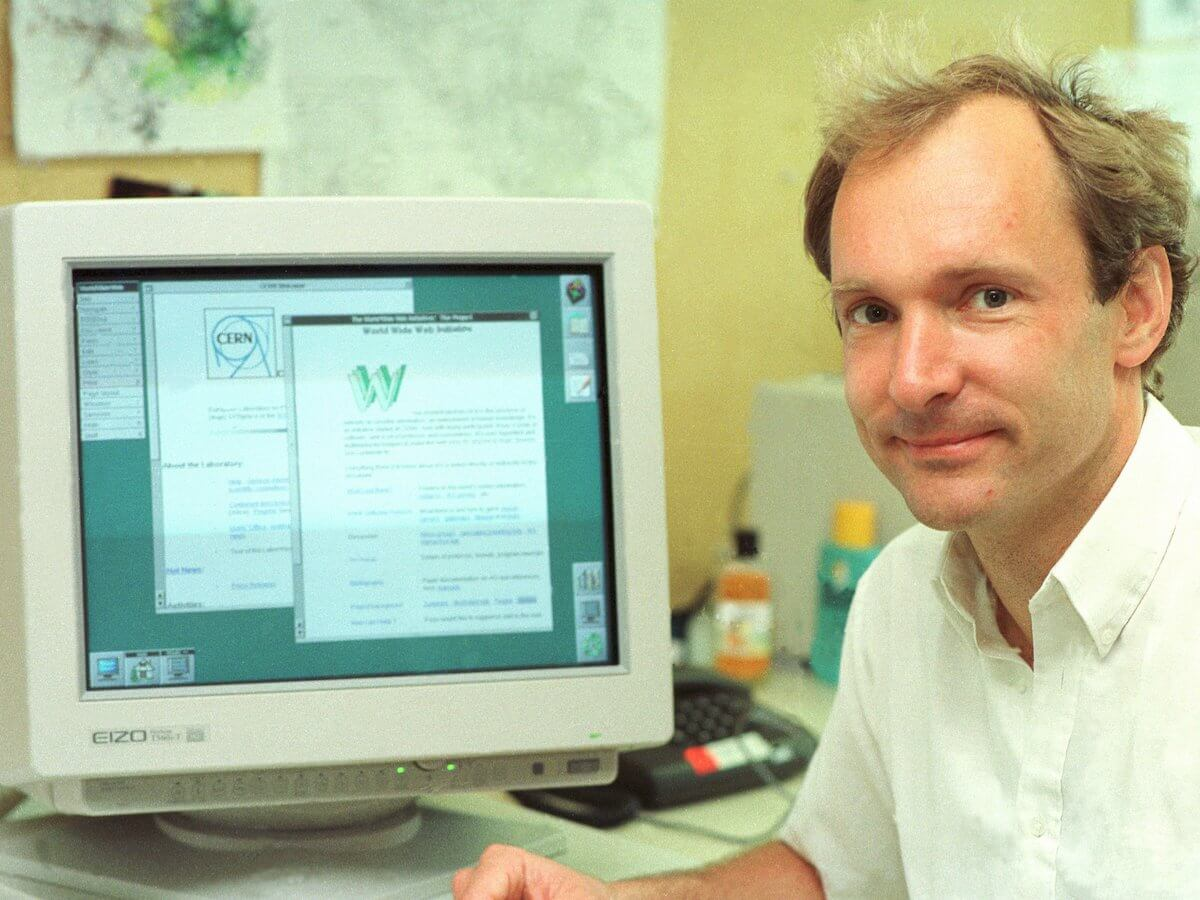
\includegraphics[width=0.45
	\textwidth,  keepaspectratio]{img/Berners-Lee}
\end{figure}
6 agosto 1991: invenzione del World Wide Web.

\smallskip

``\emph{Ho immaginato il Web come una piattaforma aperta che avrebbe permesso a tutti, ovunque, di condividere informazioni, di accedere ad opportunità e di collaborare attraverso differenti aree geografiche e confini culturali}"\\Sir Tim Berners-Lee.
}

\frame{
\frametitle{Problemi del Web secondo Sir Tim Berners-Lee}

\begin{beamerboxesrounded}[shadow=true]{Three challenges for the Web, according to its inventor}
\begin{enumerate}
	\item We've lost control of our personal data
	\item It's too easy for misinformation to spread on the Web
	\item Political advertising online needs transparency and understanding
\end{enumerate}
\end{beamerboxesrounded}
}

\frame{
\frametitle{Problemi relativi alla centralizzazione dei dati}

\begin{beamerboxesrounded}[shadow=true]{Quando i dati sono salvati in piattaforme
		digitali chiuse e centralizzate:}
	\begin{enumerate}
		\item Nessuna visibilità su ciò che viene conservato
		\item Scarso controllo su come i dati vengono utilizzati
		\item Non si può scegliere quali applicazioni usare per accedervi
		\item Non si possono usare i dati come unità coesiva
	\end{enumerate}
\end{beamerboxesrounded}

\bigskip
\textbf{$=>$ Nascita di una nuova tecnologia per ridecentralizzare il Web.}
}

\frame{
\frametitle{Solid}
\begin{figure}
	\centering
	\includegraphics[width=0.25
	\textwidth,  keepaspectratio]{img/Solid}
\end{figure}
Progetto voluto da Tim Berners-Lee e sostenuto da molti esperti di Sicurezza Informatica e del Semantic Web.

\bigskip

\textbf{Obiettivo}: ridecentralizzare il World Wide Web limitando il monopolio dei dati dell'utente.
}

\frame{
\frametitle{Concetti chiave relativi alla tecnologia Solid}
	
\textbf{Solid} permette agli utenti di salvare i propri dati in stores decentralizzati chiamati \textbf{Pod}. Ogni utente può decidere quali altre persone e applicazioni possano accedervi, concedendo loro, o eventualmente revocando loro, diritti su una risorsa/e contenuta/e all'interno del \textbf{Pod}.
	
\bigskip
	
Possibilità di concedere diversi livelli di permesso: \textbf{Read}, \textbf{Append}, \textbf{Write}, \textbf{Control}.
}

\frame{
\frametitle{Concetti chiave relativi alla tecnologia Solid}
	
\begin{beamerboxesrounded}[shadow=true]{Termini legati alla tecnologia Solid}
	\begin{enumerate}
		\item \textbf{Pod}: Luogo per salvare dati dell'utente
		\item \textbf{webId}: Identificatore univoco utente
		\item \textbf{Solid Identity Provider}: Compagnia che permette di autenticarsi e ospitare Pod
		\item \textbf{Container}: "Directory" all'interno del Pod
		\item \textbf{SolidDataset}: Dataset contente informazioni appartenenti all'utente
	\end{enumerate}
\end{beamerboxesrounded}
	
}
\frame{
\frametitle{Obiettivi della tesi}
\textbf{1) Creazione di un'applicazione completamente decentralizzata in accordo con la tecnologia Solid.}

\bigskip

Per permettere ad utenti di creare/gestire un proprio blog personale.

\bigskip

L'applicazione è stata denominata \textbf{my-solid-blog}.
}

\frame{
\frametitle{Obiettivi della tesi}
\textbf{2) Dimostrare l'utilità e l'importanza di tale tecnologia.}

\medskip
Alcuni vantaggi:
\begin{itemize}
	\item Controllo dei propri dati
	\item Arginato problema della disinformazione
	\item Evitare forme di censura
\end{itemize}

\bigskip

\textbf{Creata applicazione blog-validator per controllare autenticità dei dati dell'utente.}
}

\frame{
\frametitle{Il sistema SADeB}
Tesi finalizzata allo sviluppo di due applicazioni, \textbf{my-solid-blog} e \textbf{blog-validator}, facenti parte del sistema denominato \textbf{SADeB}.
}

\frame{
\frametitle{Anteprima my-solid-blog}
\begin{figure}
	\centering
	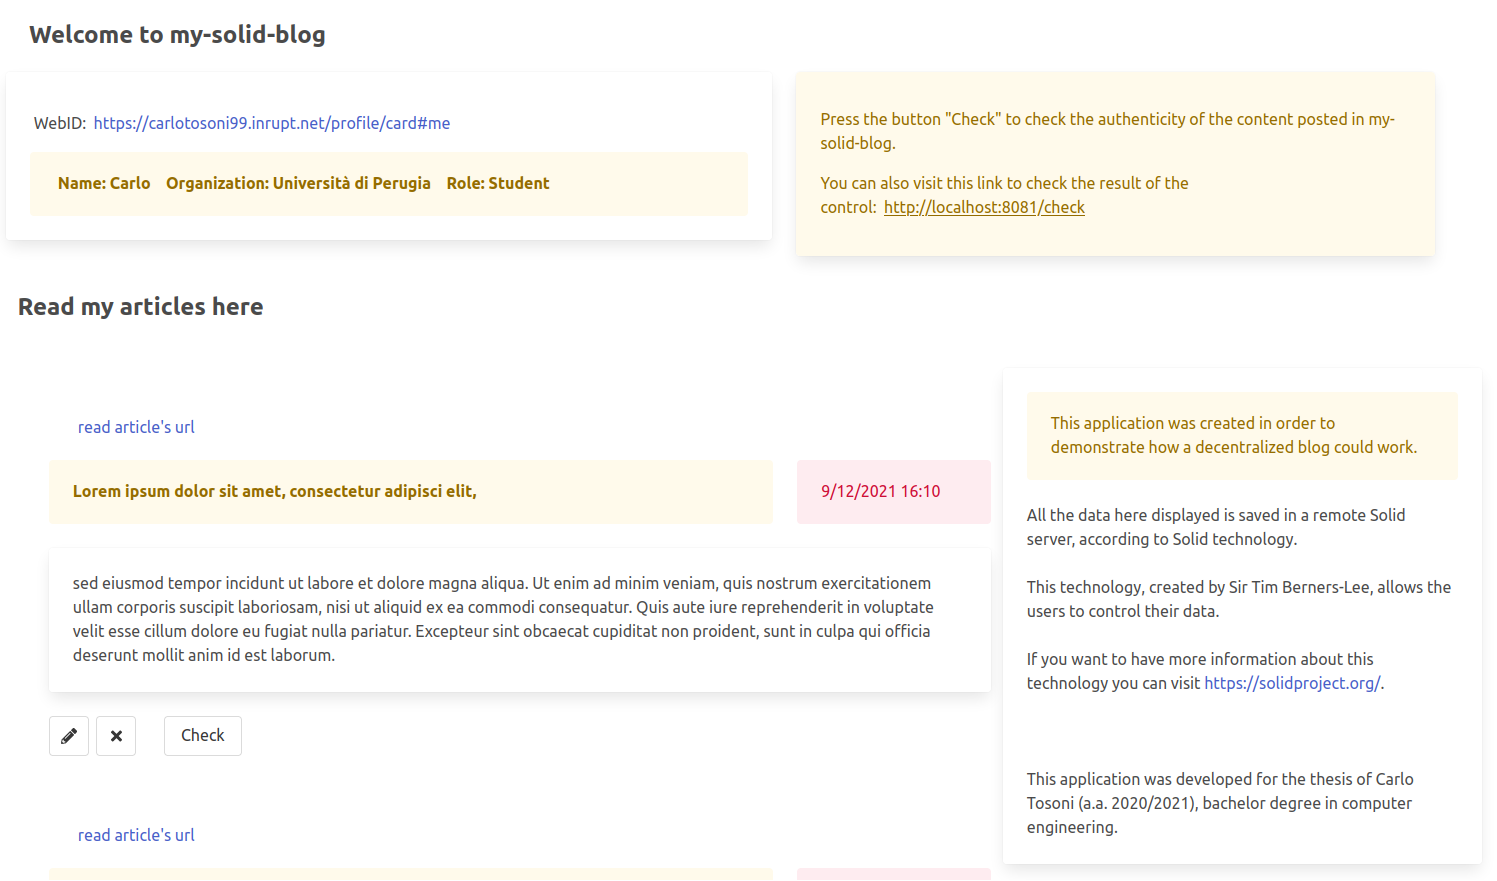
\includegraphics[width=1.0
	\textwidth,  keepaspectratio]{img/mySolidBlogUI}
\end{figure}
}

\frame{
\frametitle{Dati contenuti nel Pod}
\begin{figure}
	\centering
	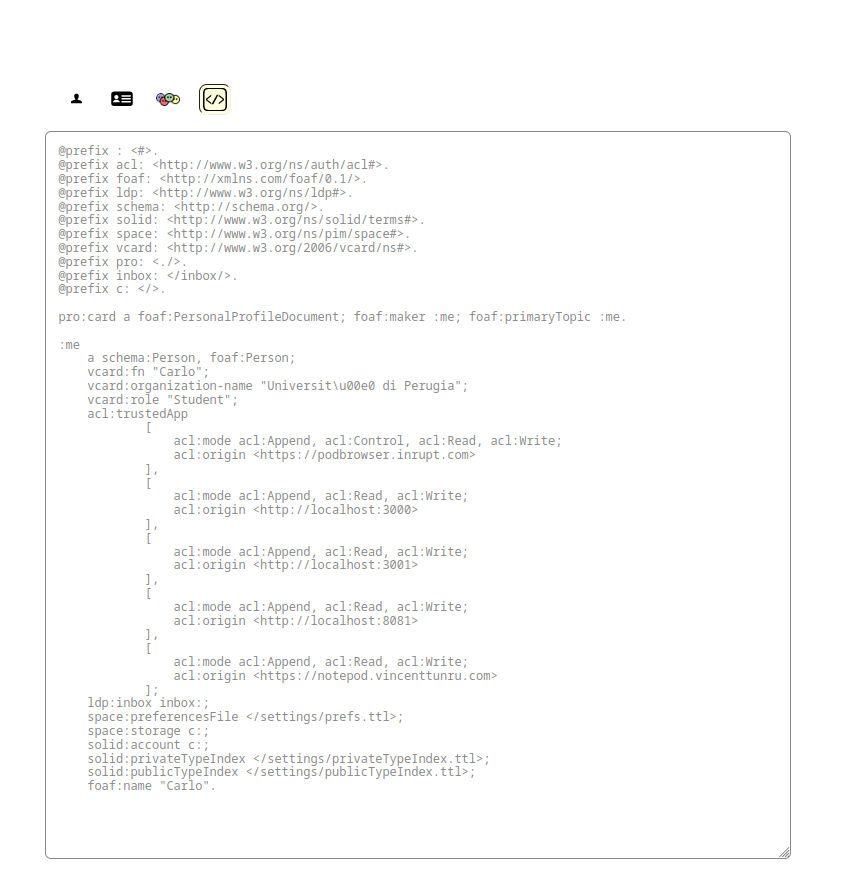
\includegraphics[width=0.6
	\textwidth,  keepaspectratio]{img/PodRDF}
\end{figure}
}



\section{Requisiti}
\frame{
\frametitle{Requisiti}
Requisiti delle applicazioni facenti parte del sistema \textbf{SADeB}.
	
\bigskip
	
\textbf{my-solid-blog:}
	
\begin{itemize}
	\item Applicazione completamente decentralizzata
	\item Possibilità di creare/gestire il proprio blog
	\item Permettere di leggere blog di altri utenti (inserendo webId proprietario)
	\item Verificare autenticità contenuti postati
\end{itemize}
}

\frame{
\frametitle{Requisiti}
Requisiti delle applicazioni facenti parte del sistema \textbf{SADeB}.
	
\bigskip
	
\textbf{blog-validator:}
	
\begin{itemize}
	\item Server per controllare autenticità dei contenuti postati
	\item Possibilità per l'utente di verificare personalmente esito controllo
\end{itemize}
}

\section{Architettura del sistema}
\frame{
\frametitle{Architettura del sistema}

Tecnologie utilizzate per lo sviluppo delle due applicazioni:

\begin{beamerboxesrounded}[shadow=true]{\textbf{my-solid-blog}}
	\begin{enumerate}
		\item \textbf{Inrupt}: Librerie JavaScript create dalla società Inrupt, fondata da Berners-Lee per gestire dati all'interno del Pod
		\item \textbf{React}: Libreria open-source, front-end, JavaScript
		\item \textbf{Bulma}: Framework CSS open-source
	\end{enumerate}
\end{beamerboxesrounded}

\medskip

\begin{beamerboxesrounded}[shadow=true]{\textbf{blog-validator}}
	\begin{enumerate}
		\item \textbf{Node.js}: Runtime system multipiattaforma orientato agli eventi
	\end{enumerate}
\end{beamerboxesrounded}
}

\frame{
\frametitle{my-solid-blog}

\begin{figure}
	\centering
	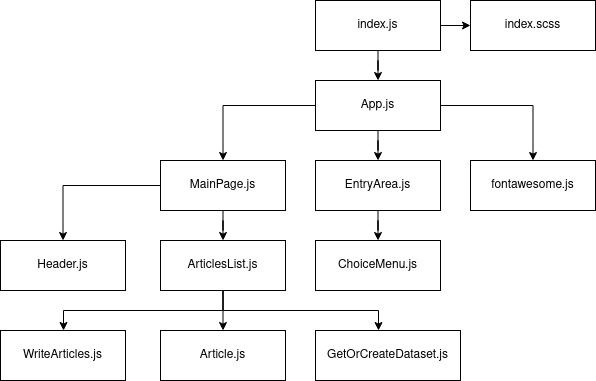
\includegraphics[width=0.7
	\textwidth,  keepaspectratio]{img/Dependencies}
\end{figure}

L’albero delle dipendenze dei moduli di \textbf{my-solid-blog}.
}

\frame{
\frametitle{my-solid-blog}
	
\begin{figure}
	\centering
	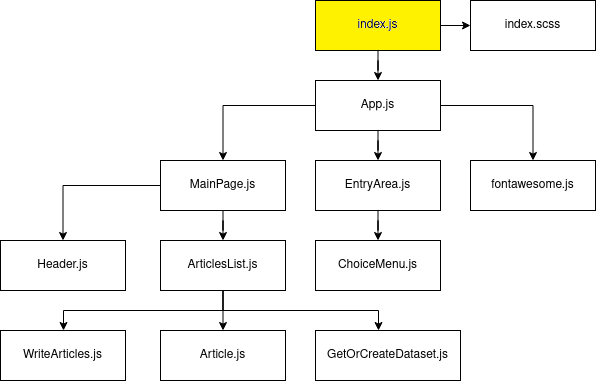
\includegraphics[width=0.7
	\textwidth,  keepaspectratio]{img/Dependencies1}
\end{figure}
	
\textbf{index.js}: Entry point di JavaScript.
}

\frame{
\frametitle{my-solid-blog}
	
\begin{figure}
	\centering
	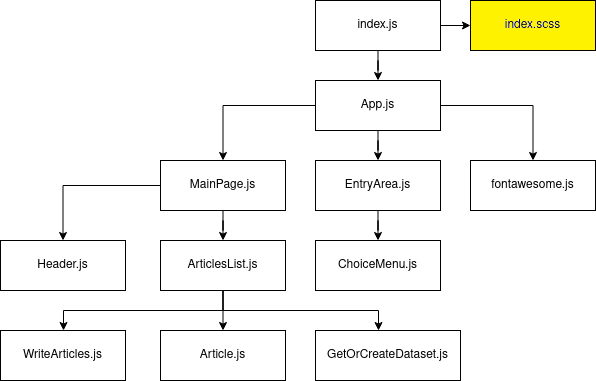
\includegraphics[width=0.7
	\textwidth,  keepaspectratio]{img/Dependencies2}
\end{figure}
	
\textbf{index.scss}: Importa componenti del framework Bulma per la formattazione del documento HTML.
}

\frame{
\frametitle{my-solid-blog}
	
\begin{figure}
	\centering
	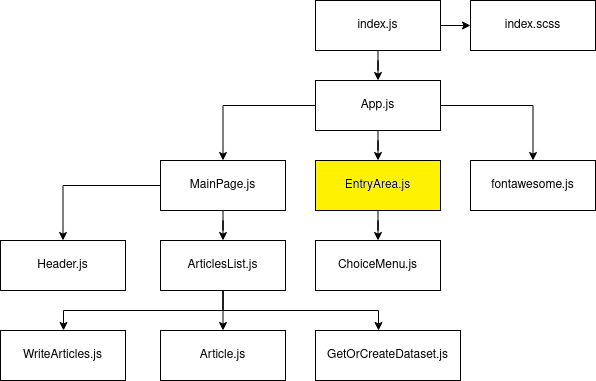
\includegraphics[width=0.7
	\textwidth,  keepaspectratio]{img/Dependencies3}
\end{figure}
	
\textbf{EntryArea.js}: Renderizza schermata prima di effettuare l'accesso. Permette autenticazione con \textbf{Solid-Identity-Provider}, oppure inserimento della \textbf{webId} del proprietario del blog.
}

\frame{
\frametitle{my-solid-blog}
	
\begin{figure}
	\centering
	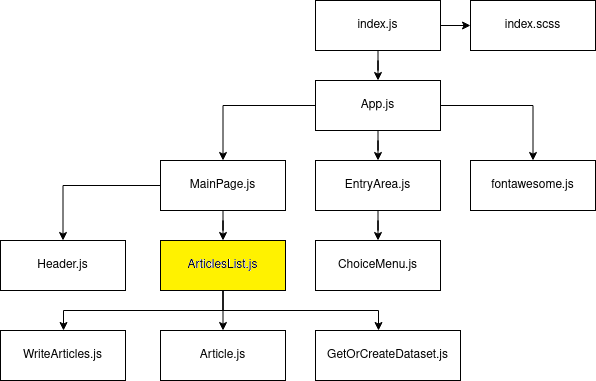
\includegraphics[width=0.7
	\textwidth,  keepaspectratio]{img/Dependencies4}
\end{figure}
	
\textbf{Articlelist.js}: Si occupa di renderizzare il contenuto di un blog e di elaborare le informazioni contenute all'interno del \textbf{SolidDataset} ove è salvato.
}

\frame{
\frametitle{my-solid-blog}
	
\begin{figure}
	\centering
	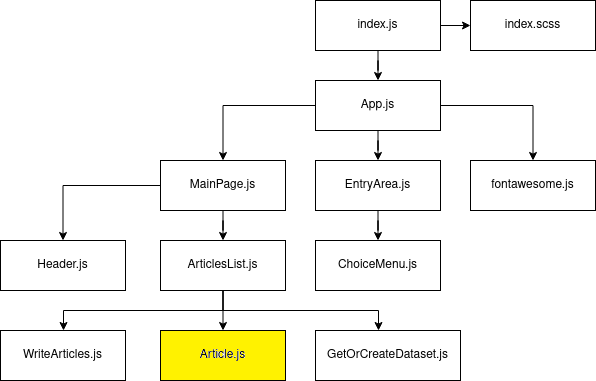
\includegraphics[width=0.7
	\textwidth,  keepaspectratio]{img/Dependencies5}
\end{figure}
	
\textbf{Article.js}: Renderizza il contenuto dei singoli articoli del blog.
}

\frame{
\frametitle{my-solid-blog}
	
\begin{figure}
	\centering
	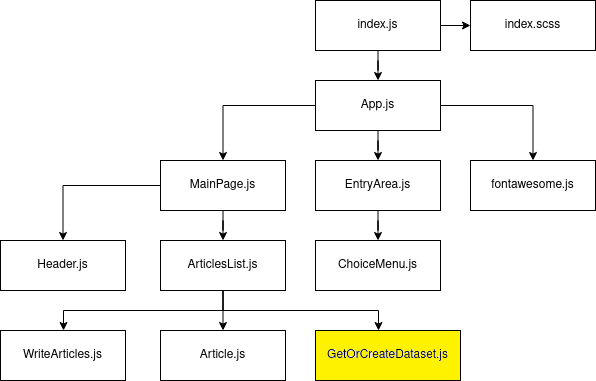
\includegraphics[width=0.7
	\textwidth,  keepaspectratio]{img/Dependencies6}
\end{figure}
	
\textbf{GetOrCreateDataset.js}: Si occupa dell'interazione con il \textbf{Pod} per quanto concerne il caricamento del \textbf{SolidDataset} contente il blog dell'utente. Qualora tale \textbf{SolidDataset} non esista, lo inizializza.
}

\frame{
\frametitle{my-solid-blog}

\textbf{Autenticazione con il Solid-Identity-Provider}

\begin{figure}
	\centering
	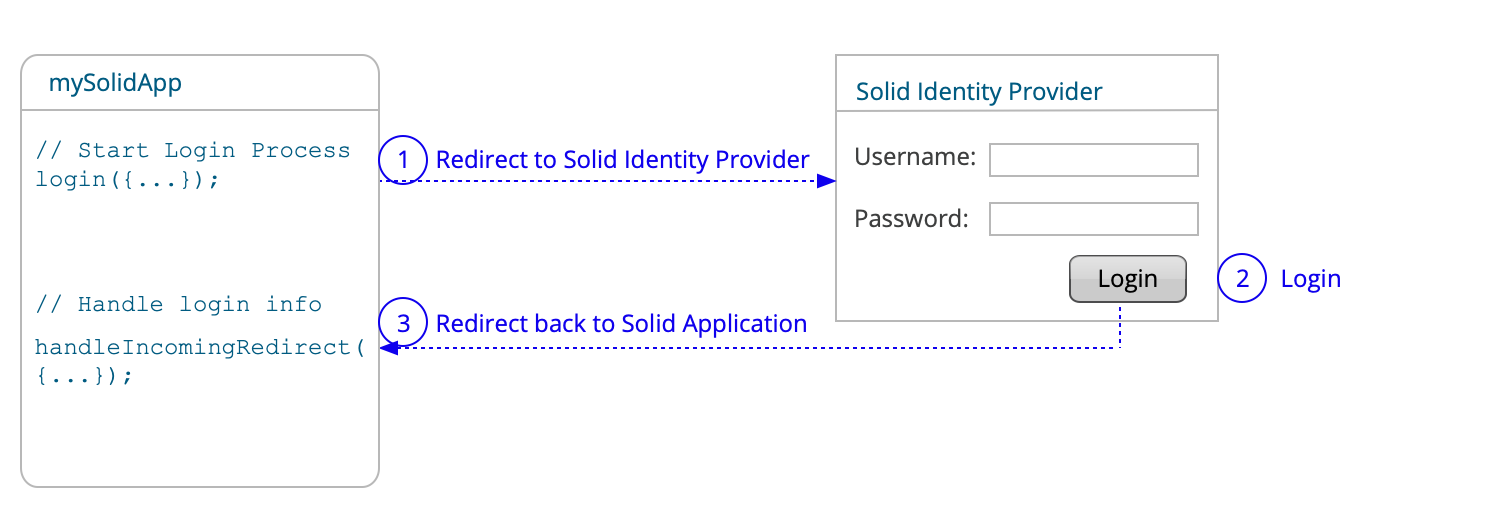
\includegraphics[width=1.1
	\textwidth,  keepaspectratio]{img/autenticazione}
\end{figure}

Autenticazione con il proprio Solid-Identity-Provider implementata tramite libreria \textbf{Inrupt} solid-ui-react.
}

\frame{
\frametitle{my-solid-blog}

\textbf{Gestione dei dati all'interno del Pod}

\bigskip

Ogni applicazione deve potenzialmente accedere ai dati contenuti all'interno del Pod. Necessaria modalità unica per la rappresentazione dei dati. Utilizzato linguaggio \textbf{RDF}.
}

\frame{
\frametitle{Resource Description Framework}

\begin{figure}
	\centering
	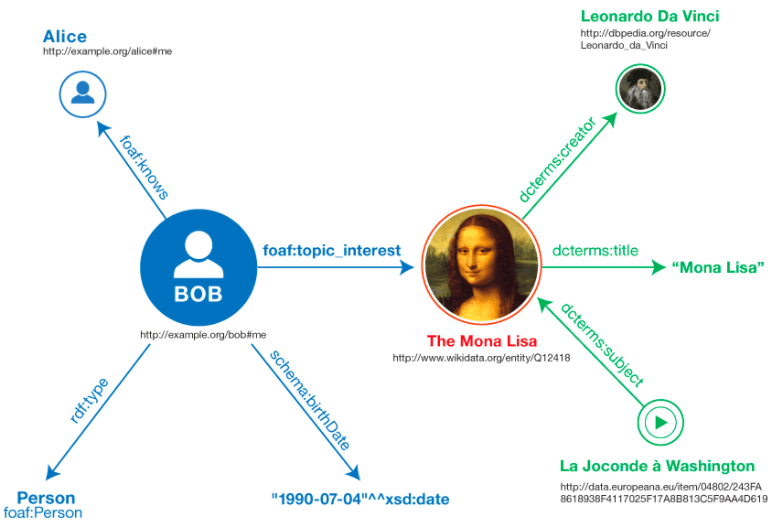
\includegraphics[width=0.53
	\textwidth,  keepaspectratio]{img/linkedData}
\end{figure}

Qualsiasi dato in \textbf{RDF} è una risorsa rappresentata tramite un \textbf{IRI}, pertanto è reperibile direttamente dal Web. Utilizzati diversi vocabolari per la rappresentazione di differenti tipologie di dati.
}

\frame{
\frametitle{Resource Description Framework}

\begin{beamerboxesrounded}[shadow=true]{\textbf{Importanti vocabolari RDF}}
	\begin{enumerate}
		\item \textbf{RDF}: Vocabolario fondamentale, definisce un modello per la rappresentazione
		dati in RDF
		\item \textbf{FOAF}: Per rappresentare persone, organizzazioni e interazioni sociali
		\item \textbf{ACL}: Vocabolario per la gestione dei livelli di accesso di un agente su una risorsa
		\item \textbf{Schema}: Definisce varie strutture di dati
	\end{enumerate}
\end{beamerboxesrounded}
}

\frame{
\frametitle{Resource Description Framework}
\textbf{Linked Data}

\smallskip

\textbf{RDF} rappresenta tuttle le informazioni tramite \textbf{Statements}. \textbf{Statements} formati da: \textbf{Soggetto}, \textbf{Predicato} e \textbf{Oggetto}.

\bigskip
\small


$<https://carlotosoni99.inrupt.net/profile/card\#me>$ sogg.\\
$<http://xmlns.com/foaf/0.1/name>$ pred.\\
$”Carlo”$ ogg.
}

\frame{
\frametitle{my-solid-blog}
Utilizzata libreria \textbf{Inrupt} \textbf{solid-client} per gestione dati nel Pod. Contenuto blog rappresentato da un \textbf{SolidDataset} chiamato \textbf{articlelist.ttl}. Ogni articolo del blog è un oggetto \textbf{RDF}.

\medskip

\begin{enumerate}
	\item Caricamento \textbf{SolidDataset} dal \textbf{Container} ove è contenuto
	\item Creazione/Modifica/Rimozione di uno o più oggetti \textbf{RDF} contenuti nel \textbf{SolidDataset}
	\item Salvataggio del nuovo \textbf{SolidDataset} all'interno del \textbf{Pod}
\end{enumerate}
}

\frame{
\frametitle{my-solid-blog}

\textbf{Codice per il caricamento del SolidDataset.}

\bigskip

\begin{figure}
	\centering
	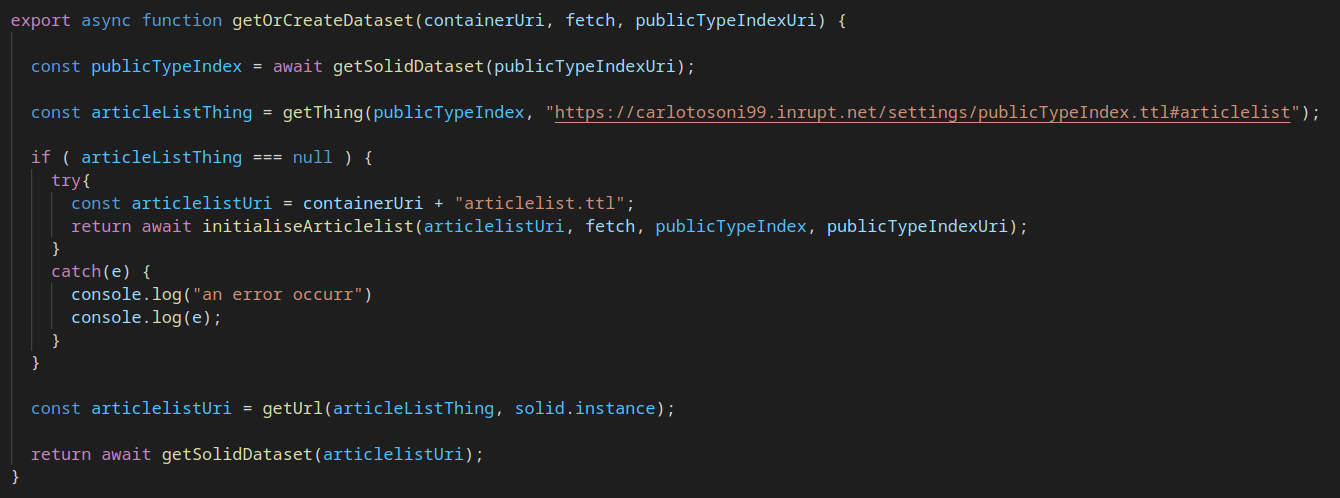
\includegraphics[width=1.05
	\textwidth,  keepaspectratio]{img/codiceDataset}
\end{figure}
}

\frame{
\frametitle{my-solid-blog}

I singoli articoli contenuti all'interno del blog sono stati definiti tramite il vocabolario \textbf{Schema}. Ogni articolo è un oggetto \textbf{RDF} appartenente alla classe \textbf{TextDigitalDocument}.

\medskip

Proprietà utilizzate:
\small

\begin{itemize}
	\item \textbf{dataCreated}: Data creazione articolo
	\item \textbf{headline}: titolo articolo
	\item \textbf{text}: contenuto articolo
	\item \textbf{identifier}: identificatore univoco articolo
\end{itemize}
}

\frame{
\frametitle{blog-validator}

Per evitare diffusione di disinformazione o forme di censura da parte di my-solid-blog, è stata creata una seconda applicazione, esterna alla prima, chiamata \textbf{blog-validator}.

\bigskip

\textbf{blog-validator} effettua dei controlli sull'autenticità dei contenuti mostrati su richiesta dell'utente.
}

\frame{
\frametitle{blog-validator}

\begin{figure}
	\centering
	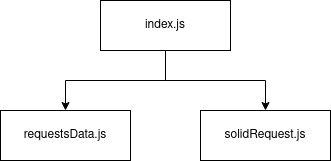
\includegraphics[width=0.5
	\textwidth,  keepaspectratio]{img/blogValidatorModules}
	
	\bigskip
	\bigskip
	
	L'albero delle dipendenze dei moduli di \textbf{blog-validator}.
\end{figure}
}

\frame{
\frametitle{blog-validator}

\textbf{I moduli di blog-validator}

\small
\begin{itemize}
	\item \textbf{index.js}: Entry point di JavaScript, definisce le \textbf{API methods} necessarie per effettuare controlli sull'autenticità dei dati mostrati da \textbf{my-solid-blog}, e per permettere all'utente di verificare personalmente l'esito di tali controlli
	\item \textbf{solidRequest.js}: Legge i dati relativi al blog all'interno del \textbf{Pod} dell'utente, per confrontarli con quelli ricevuti da \textbf{my-solid-blog}
	\item \textbf{requestsData.js}: Memorizza in un database locale i dati relativi alle richieste di controllo dei dati mostrati da \textbf{my-solid-blog} per visualizzarli all'utente qualora questo ne richieda la visione, per la gestione del database utilizza la libreria \textbf{sqlite3}
\end{itemize}
}

\frame{
\frametitle{Comunicazione tra le due applicazioni}

La comunicazione tra \textbf{my-solid-blog} e \textbf{blog-validator} avviene tramite protocollo \textbf{HTTP}. Premendo il pulsante "Check", \textbf{my-solid-blog} invia una richiesta \textbf{POST} al server \textbf{blog-validator}, contenente tutti i parametri necessari per effettuare un controllo sui dati.
}

\frame{
\frametitle{Parametri passati a blog-validator per il controllo}

\small
\begin{enumerate}
	\item \textbf{webId}: WebId del proprietario dell'articolo
	\item \textbf{urlDataset}: URL del \textbf{SolidDataset} contenente l'articolo
	\item \textbf{urlThing}: URL dell'articolo
	\item \textbf{title}: Titolo dell'articolo
	\item \textbf{content}: Contenuto dell'articolo
	\item \textbf{date}: Data di creazione dell'articolo
\end{enumerate}

Usata libreria \textbf{axios} per stabilire comunicazione \textbf{HTTP}.

\bigskip

\textbf{my-solid-blog} utilizza la porta \textbf{3000}, mentre \textbf{blog-validator} la porta \textbf{8081}.
}

\section{Esempi di utilizzo}
\frame{
\frametitle{Avvio my-solid-blog}
	
\begin{figure}
	\centering
	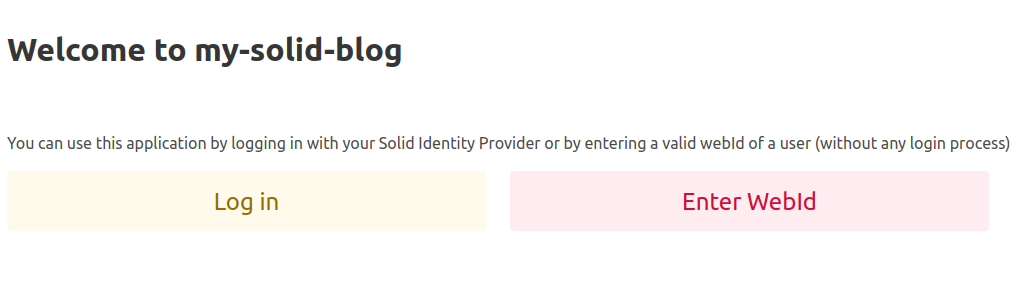
\includegraphics[width=1.
	\textwidth,  keepaspectratio]{img/Choice}
\end{figure}
}

\frame{
\frametitle{Interfaccia my-solid-blog}

\begin{figure}
	\centering
	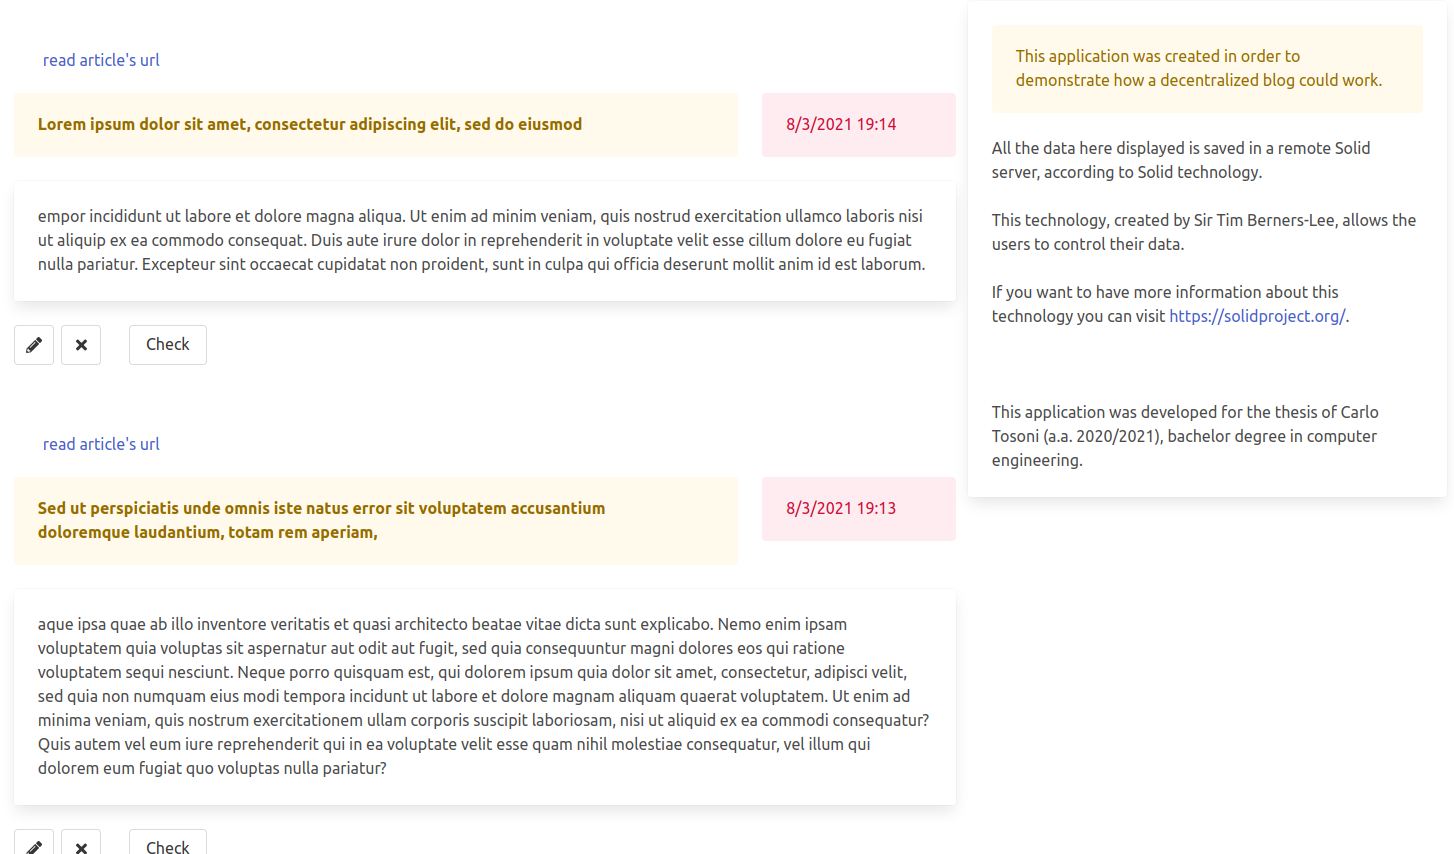
\includegraphics[width=1.0
	\textwidth,  keepaspectratio]{img/blogArticles}
\end{figure}

}


\frame{
\frametitle{Possibilità modifica contenuto articolo}

\begin{figure}
	\centering
	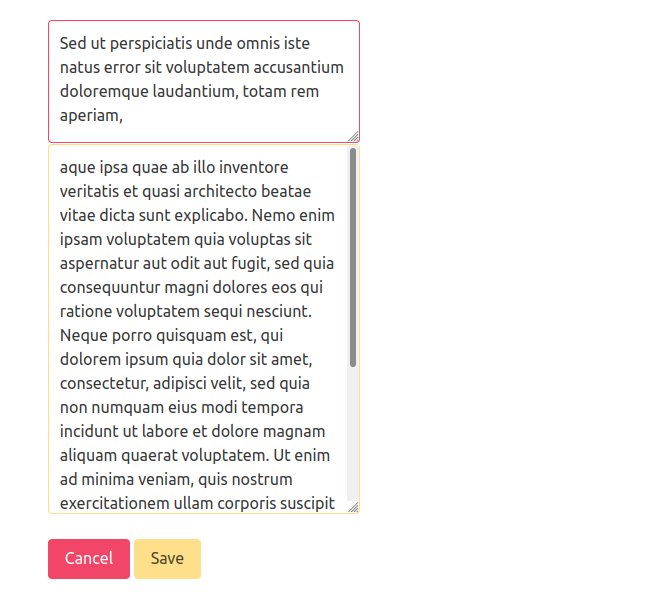
\includegraphics[width=0.65
	\textwidth,  keepaspectratio]{img/modifyArticle}
\end{figure}
}

\frame{
\frametitle{Contenuto blog in RDF}

\begin{figure}
	\centering
	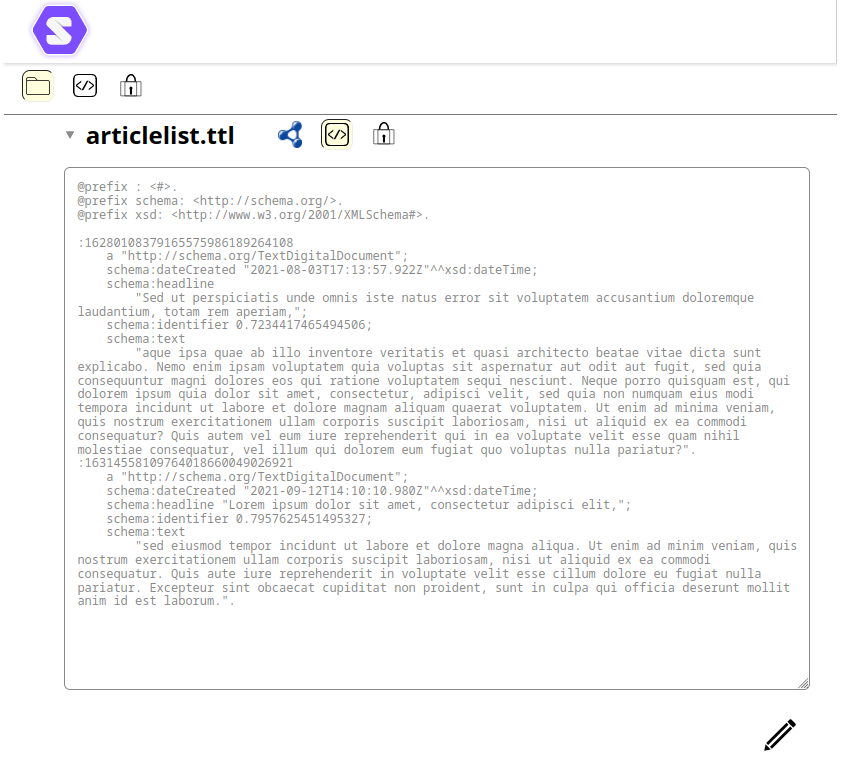
\includegraphics[width=0.65
	\textwidth,  keepaspectratio]{img/RDFBlog}
\end{figure}
}

\frame{
\frametitle{Controllo autenticità articolo}
	
\begin{figure}
	\centering
	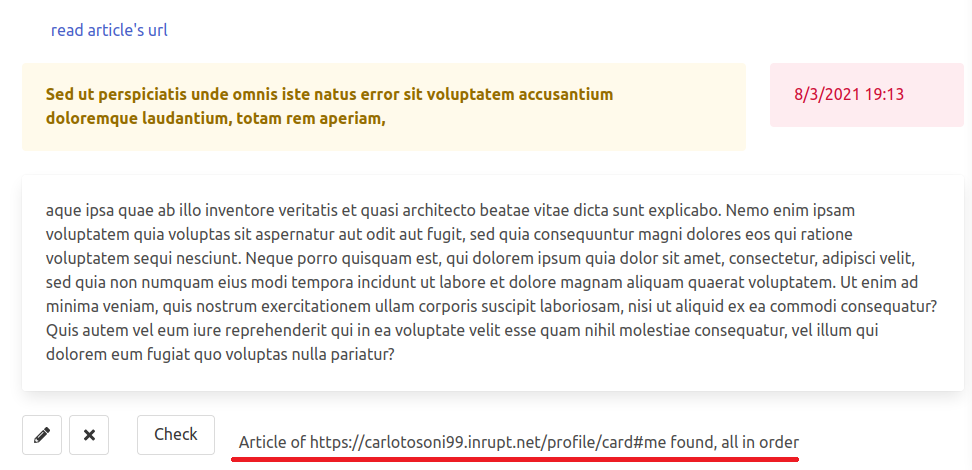
\includegraphics[width=1.0
	\textwidth,  keepaspectratio]{img/checkArticle}
\end{figure}
}

\frame{
\frametitle{blog-validator}

\begin{figure}
	\centering
	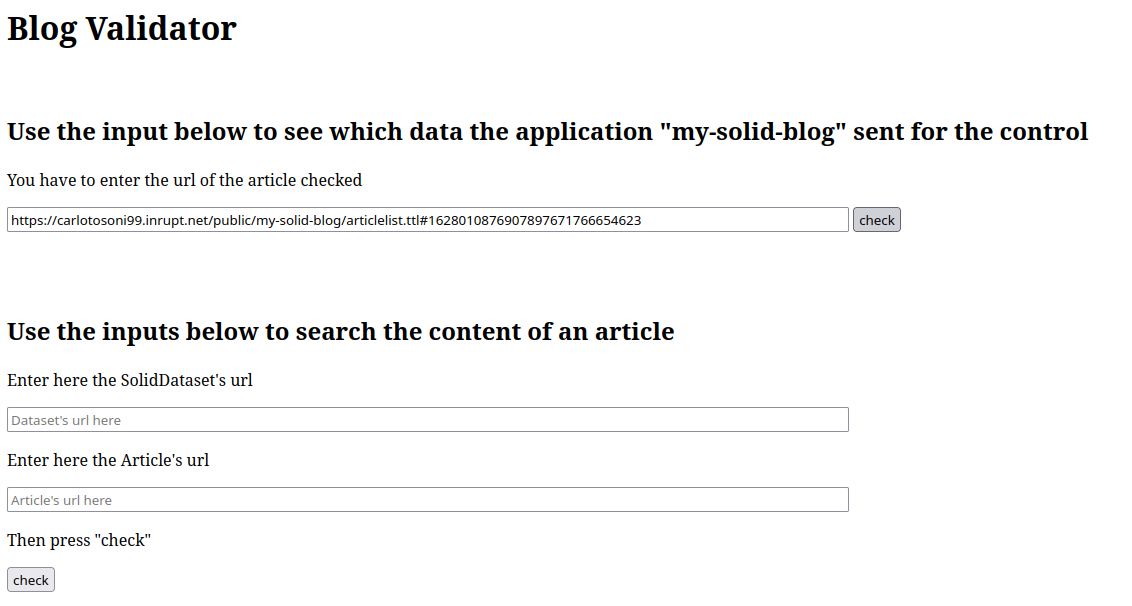
\includegraphics[width=1.0
	\textwidth,  keepaspectratio]{img/blogValidator}
\end{figure}
}

\section{Conclusioni}
\frame{
\frametitle{Conclusioni e sviluppi futuri}

\textbf{Solid}, pur essendo una tecnologia dal grande potenziale, è ancora in via di sviluppo. Pertanto alcune sue funzionalità non sono state ancora completamente definite, oppure non presentano un'adeguata documentazione.

\bigskip

A tal proposito, per esempio, nell'implementazione dell'applicazione \textbf{my-solid-blog}, vi sono stati alcuni problemi riguardanti la gestione delle risorse \textbf{ACL}, essenziali per la gestione dei livelli di accesso di un agente sulle risorse contenute all'interno del Pod.
}

\frame{
\frametitle{Conclusioni e sviluppi futuri}

\textit{``\emph{The Web Access Control specification is not yet finalised. As such, this function is still experimental and subject to change, even in a non-major release.}"}

\bigskip

Frase presente all'interno della documentazione \textbf{Inrupt}, relativa alle funzioni per la gestione delle risorse \textbf{ACL}.
}

\frame{
\frametitle{Conclusioni e sviluppi futuri}

\textbf{Solid} è una tecnologia concepita per arginare il fenomeno della eccessiva centralizzazione del Web, i dati di milioni di utenti, ottenuti in cambio di servizi gratuiti, sono in pratica "imprigionati" nei data center dai grandi giganti operanti in questo settore.

\bigskip

La tecnologia \textbf{Solid} può sicuramente mitigare questo fenomeno, ponendo le basi per lo sviluppo di piattaforme digitali ove in controllo dei dati è restituito agli utenti, riducendo il rischio di fenomeni di censura e favorendo lo sviluppo di meccanismi di validazione delle informazioni.
}

\frame{
\frametitle{Conclusioni e sviluppi futuri}

\textbf{Scandalo Facebook-Cambridge Analytica} (2018): Raccolta dei dati di 87 milioni di utenti Facebook, senza il loro consenso, per scopi di propaganda politica.

\bigskip

Forte necessità di modificare il Web al fine di decentralizzarlo.
}

\frame{
Ringrazio tutti per l'attenzione
}

\end{document}

%\section{Conclusioni}
%\frame{
%\frametitle{\textbf{Concludendo...}}
%Il lavoro di tesi si \`e articolato nelle seguenti fasi:
%\begin{enumerate}
%\item Lorem ipsum
%\item Lorem ipsum
%\item Lorem ipsum
%\end{enumerate}
%\vspace{0.1cm}
%\setbeamercolor{postit}{fg=black,bg=green} %Baloon di colore diverso, senza sfondo
%\begin{beamerboxesrounded}[upper=postit ,lower=postut ,shadow=true]{Lorem ipsum:}
%\begin{itemize}
%\item Lorem ipsum
%\item Lorem ipsum
%\end{itemize}
%\end{beamerboxesrounded}
%}


%\begin{beamerboxesrounded}[shadow=true]{Lorem ipsum?} % Baloon grafici
%Lorem ipsum:
%\begin{enumerate}
%	\item Lorem ipsum
%	\item Lorem ipsum
%\end{enumerate}
%\end{beamerboxesrounded}
